\chapter{Ensamblajes Básicos}

\begin{figure}[H]
	\centering
	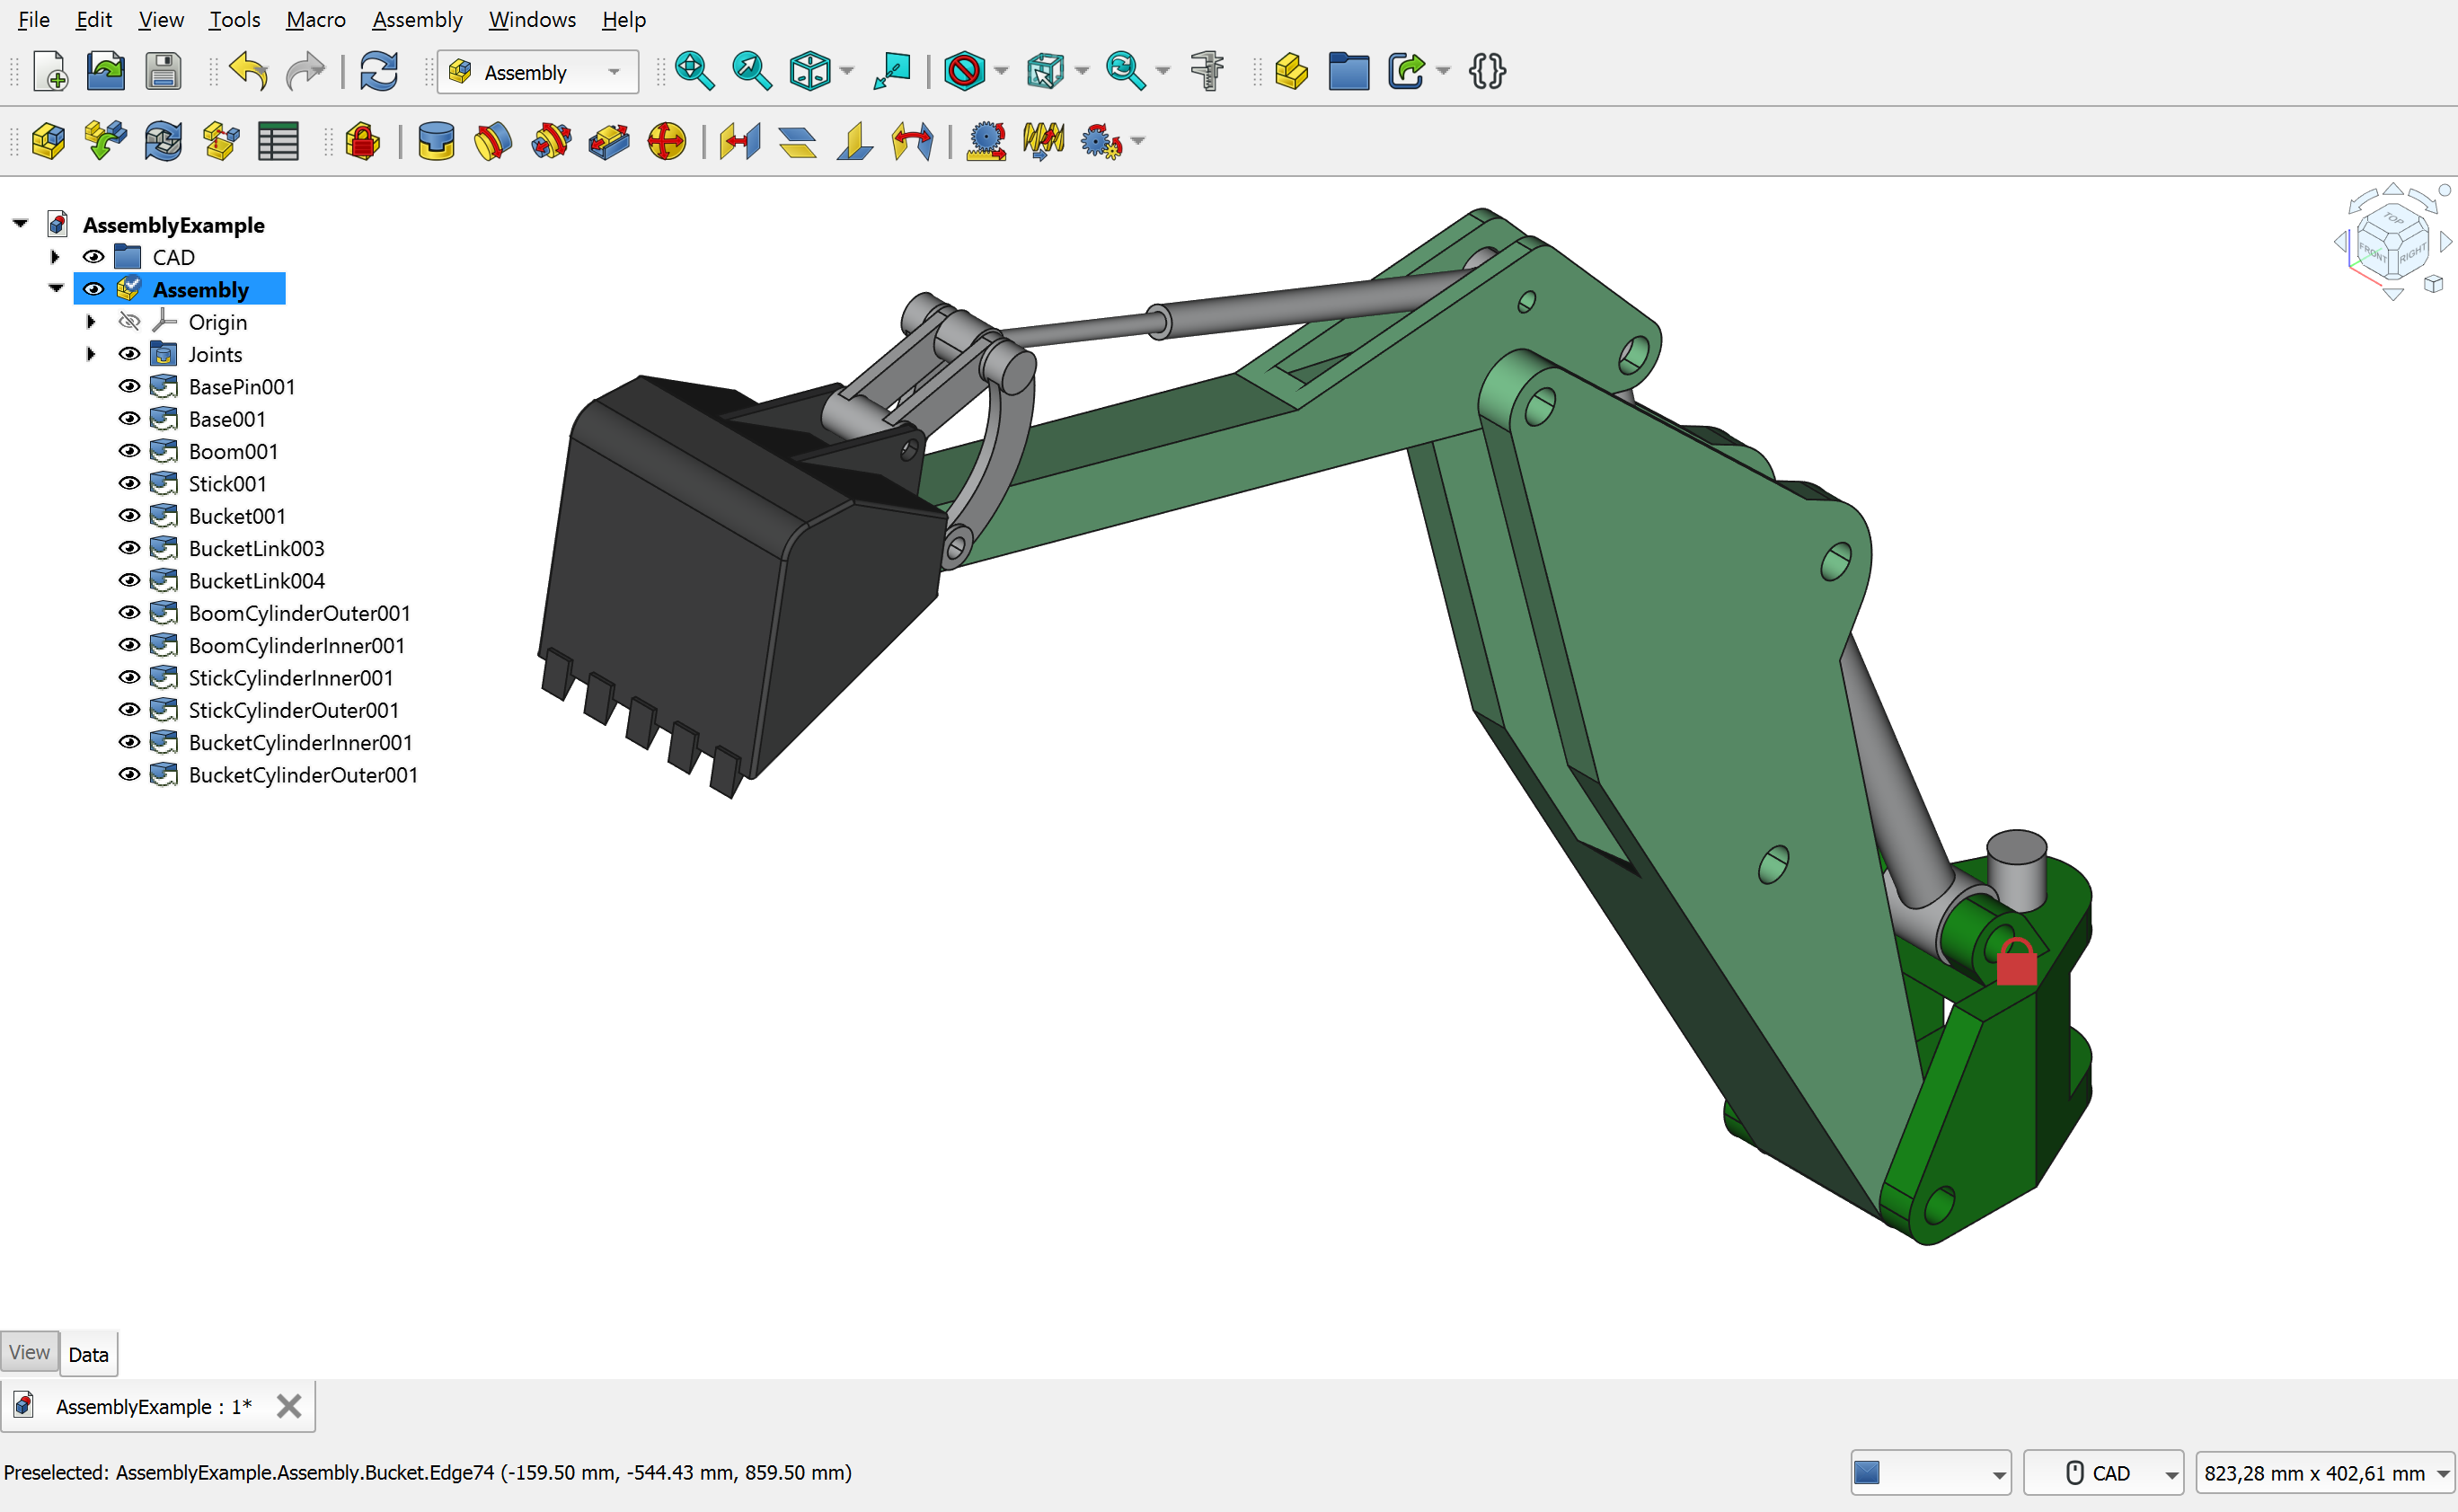
\includegraphics[width=0.8\textwidth]{img/cap9_ensamblajes.png}
	\caption{Ensamblaje de múltiples piezas en FreeCAD}
\end{figure}

Aprende a crear ensamblajes de múltiples piezas en
FreeCAD. Une componentes, define restricciones de
ensamblaje y crea mecanismos simples.

%% D. Búsqueda e Inserción de Activos Gráficos
%% Imagen insertada al inicio del capítulo

%% B. Actividades Teóricas
\section{Investigar y responder}
\faPencil

Investiga sobre ensamblajes en FreeCAD y responde:
\begin{enumerate}
	\item ¿Qué es un ensamblaje en diseño CAD?
	\item ¿Cómo se importan piezas externas en un archivo?
	\item ¿Qué tipos de restricciones de ensamblaje existen?
	\item ¿Cómo se definen relaciones de coincidencia?
	\item ¿Qué es la ``explosión'' de un ensamblaje?
	\item ¿Cómo se detectan interferencias entre piezas?
	\item ¿Qué plugins existen para ensamblajes en FreeCAD?
	\item ¿Cómo se crean listas de materiales (BOM)?
\end{enumerate}

%% C. Actividades Prácticas
\section{Resolver los siguientes problemas}
\faWrench

Problemas para aplicar conocimientos:
\begin{enumerate}
	\item Crea dos piezas simples separadas en archivos
	      diferentes.
	\item Importa ambas piezas en un nuevo archivo de
	      ensamblaje.
	\item Aplica una restricción de coincidencia entre
	      caras de las piezas.
	\item Añade una restricción de alineación entre
	      ejes de las piezas.
	\item Crea un ensamblaje de tres piezas con diferentes
	      tipos de restricciones.
	\item Practica la ``explosión'' del ensamblaje para
	      visualizar componentes.
	\item Detecta interferencias en un ensamblaje
	      mal restringido.
	\item Modifica la posición de una pieza después de
	      crear el ensamblaje.
	\item Crea un ensamblaje simple de un mecanismo
	      de biela-manivela.
	\item Exporta el ensamblaje a formato STEP para
	      intercambio con otros programas.
\end{enumerate}